
\documentclass[a4paper, 10pt, conference]{IEEEconf}  


%\usepackage{geometry}
%\geometry{a4paper, margin=1in}

\usepackage{verbatim}
\usepackage{graphicx}
\usepackage{pdfpages}
\usepackage{cite}



\setlength{\parskip}{1em}


\title{\LARGE \bf
Literature Review\\Prosthetic Tactile Sensor With Force Feedback
}

\author{Marc Alexander Sferrazza%
\thanks{*This work was not supported by any organisation}%
\thanks{Faculty of Mechatronics Engineering, Massey University, Albany, Auckland, New Zealand
        {\tt\small Progress of project: alex1v1a.github.io /Prosthetic-Tactile-Research/}}%
}


\begin{document}

\begin{figure}
	\centering
	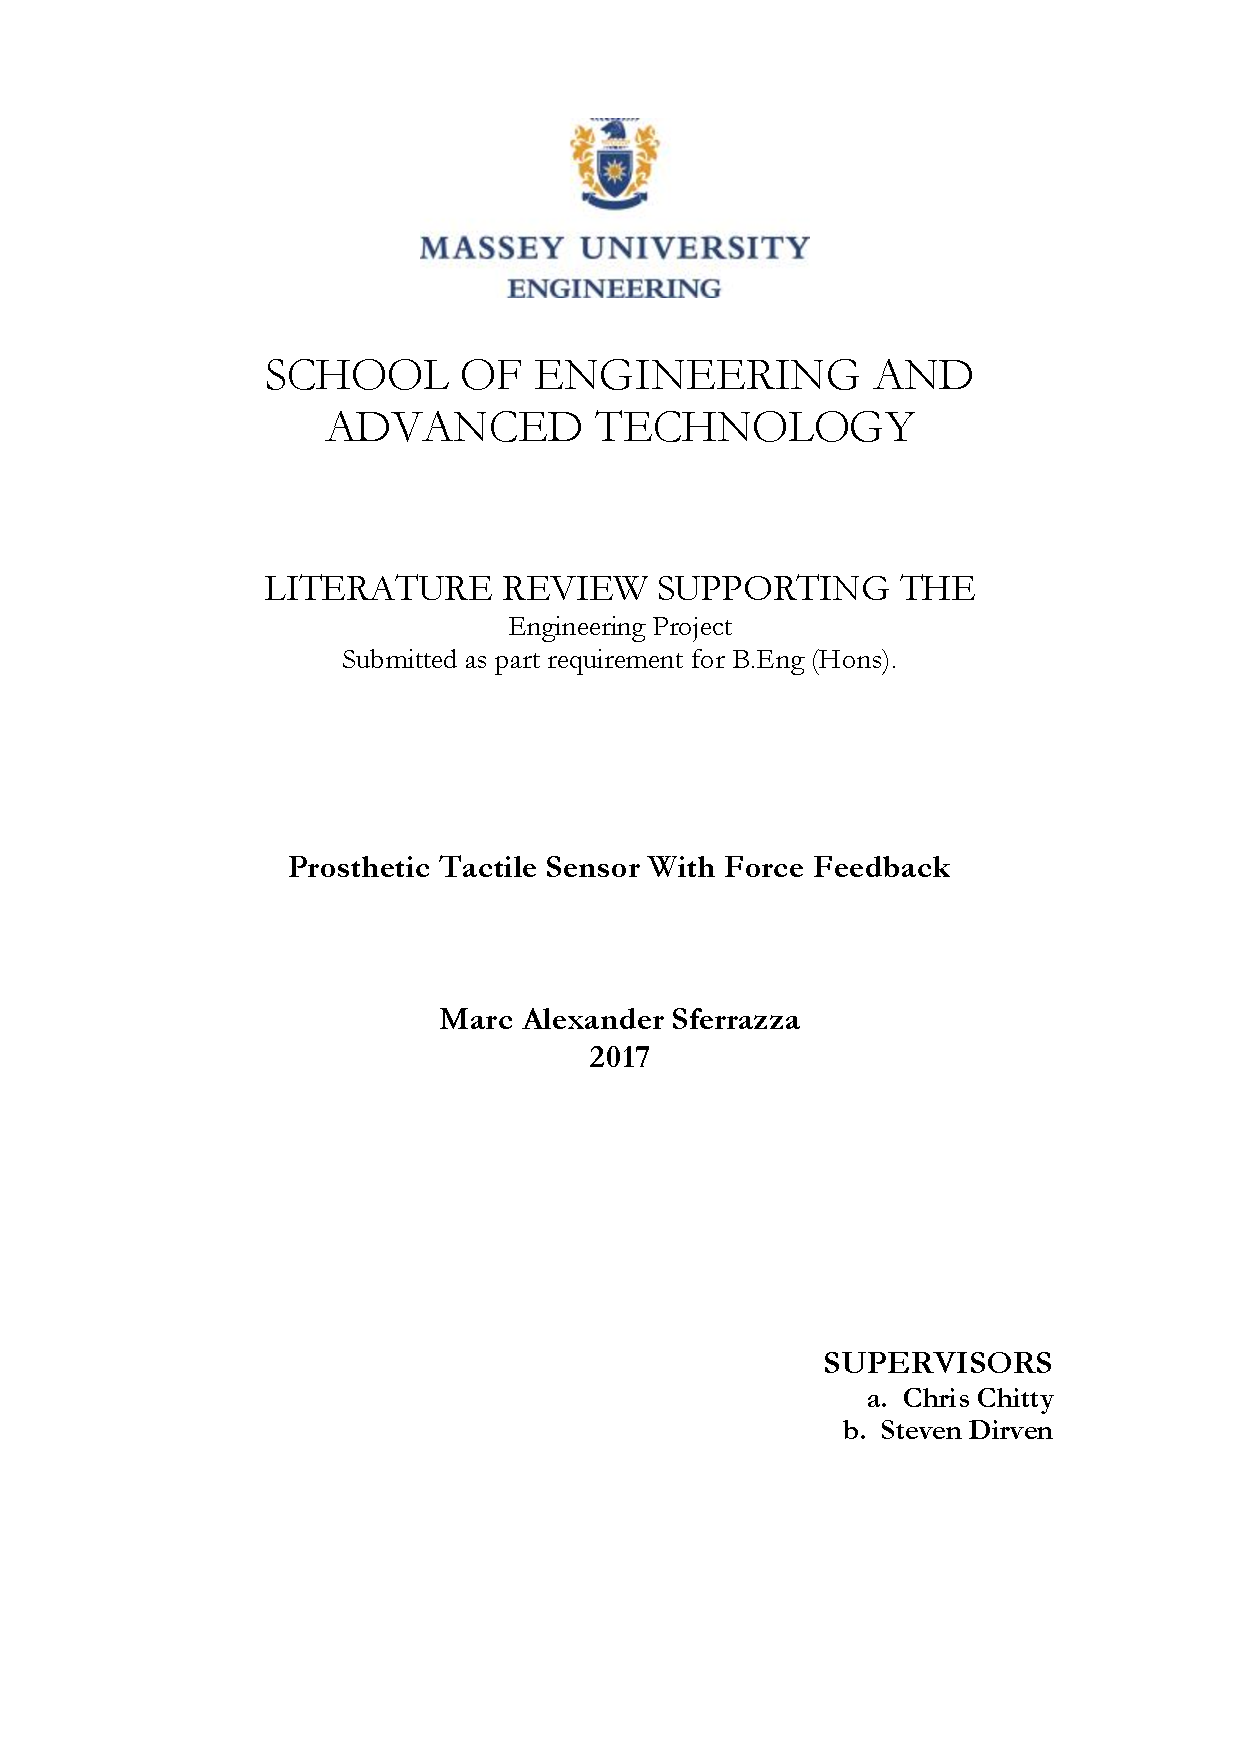
\includepdf[pages=-]{TitlePage.pdf}
\end{figure}

\
\clearpage
\tableofcontents


\maketitle
\thispagestyle{plain}
\pagestyle{plain}


\setcounter{page}{1}
%\thispagestyle{empty}
%\pagestyle{empty}


\begin{abstract}

The focus of this research is in the area of tactile sensors, and their application in the field of prosthetics. Such a study is important in order to further develop practical implementations for a forced feedback analysis, to give the sense of touch back to those whom have lost limbs. The research approach adopted in this dissertation is due to the high impact on amputees lives without the ability to feel what they are doing. 

The findings from this research provide evidence that tactile sensory is a viable force measure tool, while the range of dynamic sensory (temperature, stroking) is still limited. There are processes currently being specifically targeted in capturing this data and relaying it correctly. 

The main conclusions drawn from the study are that tactile's are a largely accepted means of measurement for prosthetics, and the methods of implementation of these sensors range immensely for applications not limited to that of this condition. 

It is found that the use of durable tactile's in an array provides a reasonable level of ranged force feedback, which in turn can be passed as output to a user to distinguish differences of sharp and smooth objects relative to this application. 

This dissertation recommends that a viable sensor for use with prosthetics will be that of a durable and high-resolution force measurement tactile which is closely meet with by E-Skin (Tokyo University Professor Takao Someya), and PRINTSKIN (Dr. Ravinder S. Dahiya, University of Glasgow Scotland).

\end{abstract}


\section{INTRODUCTION}

%Background
Tactile sensors have a wide range of applications from medical instruments, manufacturing line, sorting tasks, and much more. 

Over the last decade tactile sensors have been refined from their more rudimentary predecessors; which in turn provides far more variety of applications \cite{rogers2010materials} One opportunity opened when durable tactile's with moderate usable resolution presented itself is the task or implementation in prosthetics \cite{sekitani2008rubberlike}

%Scientific
Doctors are now successfully experimenting with a surgery called TMR (targeted muscle reinnervation) also known as TSR (targeted sensor reinnervation) with slight variances \cite{kuiken2009targeted}

This surgery unbundles the main already severed nerves (touch and muscle control) and maps them to a patients skin nerves; which allow devices such as electrodes to be used to measure the patterns and run algorithms to determine process's of movement currently up to 10 degrees of freedom [John Hopkins APL, DARPA] 

This nerve mapping stimulation of the mapped skin area could be used to give sensation back feeling in a missing limb, down to the stroke on the pinky \cite{tabot2013restoring} An additional side effect is that the mapped nerves can also sense the ranges regular appendages could, with temperature and sharpness.


%Value/significance/benefits of this research
This procedure gives users back control of a once lost limb; it also can be issued back dynamically; none the less from a stimulated force feedback, to temperature control \cite{nicolelis2002controlling} The focus of this research more specifically is in which a force is to be measured, giving an output to which can be applied to the user. 

The frame of tactile's today has come along way in the last 10 years for robotics, and can now successfully be utilised for this application \cite{someya2004large}

%Research focus
A number of methods have already been implemented in order to achieve this task. Currently there are several limitations including size, durability and deformation, types of sensors, and other aesthetic and ethic aspects to be praised \cite{collinger2013high}

\begin{figure}[h!]
  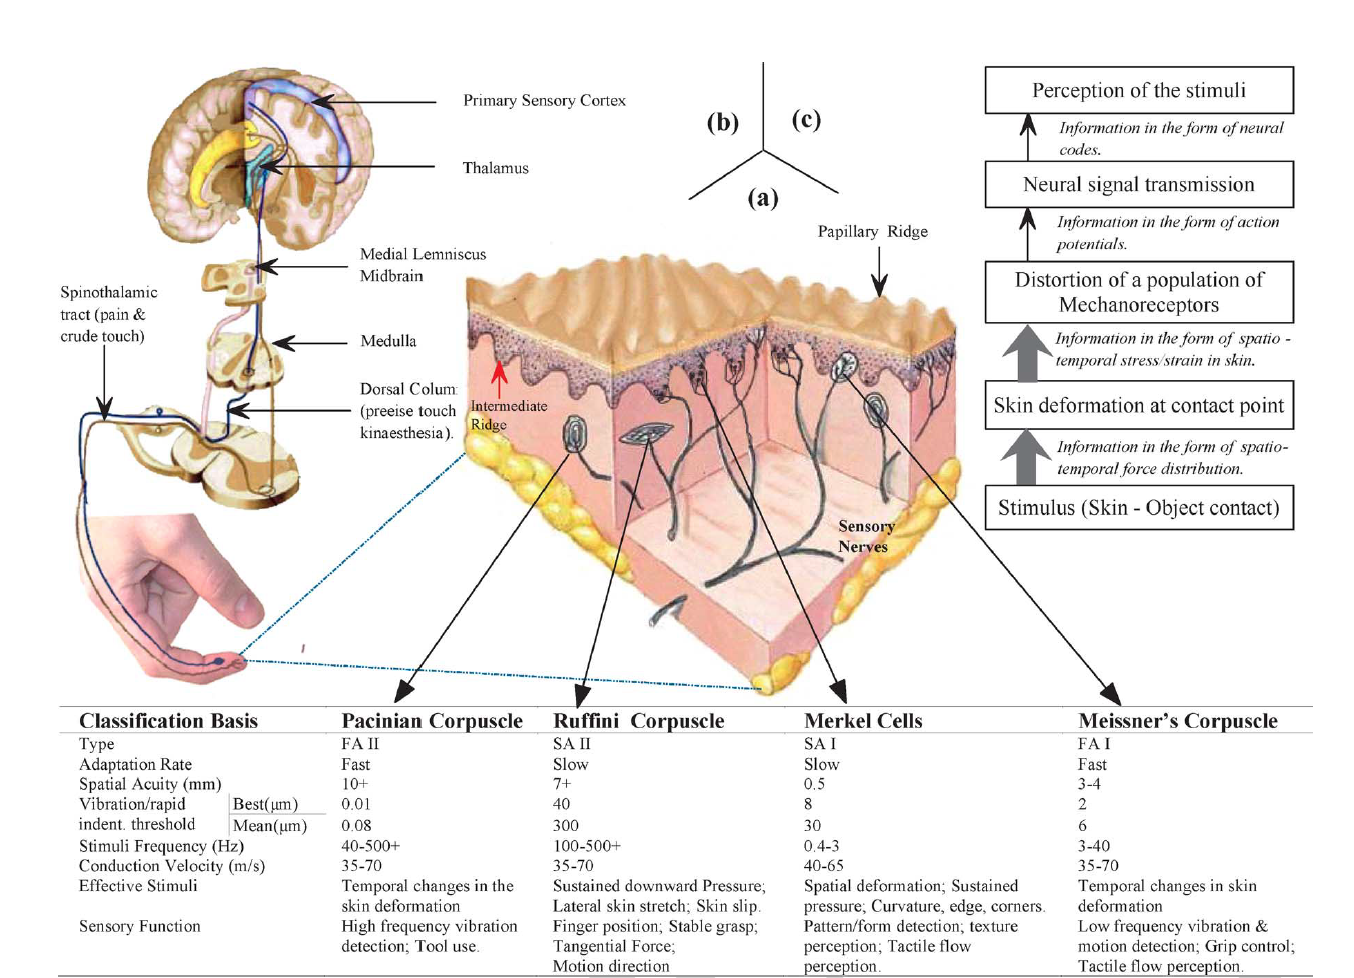
\includegraphics[width=\linewidth]{images/Nerve}
  \caption{Understanding the fundamentals; A simplified diagram of communication of the nerve connection from the brain to fingertips}
  \label{fig:Nerve}
\end{figure}

%Research aims and individual research objectives, Objectives and topics of the review relevant to this research
The main aspect to focus for this prosthetic tactile research is to apply an array of tactile's to a wearable device; in which an output can be given, such that a high enough resolution is available to determine the difference between smooth distribution and sharp surfaces e.g. a sea egg (urchin) and a chicken egg. 

This is a critical move in using a tactile device to output in micro volts and stimulate the nerve sense with the TMR mapping. \cite{collinger2013high} It is hoped to re-obtain some of the lost sense. This could be applied for machines, and patients with nerve damage not just amputees. 

It also opens the possibility in assistive touch for those suffering from muscle diseases such as ALS, in the respect that in collaboration with another device a computer is able to assist the user in not over-gripping/under-gripping of objects etc \cite{sekitani2008rubberlike}

\begin{comment}
?	A concise definition of a topic under consideration (this may be a descriptive or argumentative thesis, or proposal), as well as the scope of the related literature being investigated. (Example: If the topic under consideration is `women's wartime diaries', the scope of the review may be limited to published or unpublished works, works in English, works from a particular location, time period, or conflict, etc.)
?	The introduction should also note intentional exclusions. (Example: "This review will not explore the diaries of adolescent girls.")
?	Another purpose of the introduction is to state the general findings of the review (what do most of the sources conclude), and comment on the availability of sources in the subject area.

Introductory section
o Explain why the review is carried out
o Describe the scope of the review
o Explain how the information in the
\end{comment}

\section{Review of Literature}

Tactile force feedback is a new way to make machines aware of their surroundings and safely deform around them. They have been developed for over 30 years with the idea of first measuring pressure over a cylinders surface for LPG tanks and water cylinders. 

Since then the design has passed from capacitance and resistive measurements with simple implementations in use such as bendable resistors, surface pads, midi control tiles, pushing for smaller and smaller device applications. 

The technology has lead to developments in more sophisticated instruments, which now take advantage of more intricate designs of MOSFET's and other types of transistors; more commonly used today are POSFET's (piezoelectric polymers) 

These POSFET designs are already being used in many manufacturing devices today, and are being further developed with even smaller elements, in more durable and ductile ways; also beginning to explore the potential to simultaneously act as PV cells absorbing light efficiently.

There is a performance criteria still to be met, of which can be done with organic compounds in substitute of the current inorganic's favoured in todays POSFET's. These inorganic materials are favoured for stability, but are overwhelmed by the organics in accuracy and ductility. 

The features of organic's are highly appealing in the task at hand, however unfortunately due to the infancy of the research at this stage organics are unfeasible as to their instability.

\begin{comment}
Tracing the origin of ideas

	When and where the original discovery was made and the concepts defined

	To share appreciation for fundamental issues, principles, methods, and techniques which influenced the development of the field

Critical assessment of the state of the art

	Establishing the state-of-the-art in the field
		Approach and methodology means of discovery discovery as accepted or established by the research community
		Pros and cons in terms of a set of performance criteria
		Remaining issues and new challenges
	
	Identifying the benchmark for performance evaluation

Establishing the significance (scientific and social) and innovation of the proposed research
\end{comment}


\subsection{Technique}

This development provides wide range of innovative applications. To find more about the current technology available, checks at each point have been carefully recognised. 

With further reading analysis, breaking down the main research task into blocks and analysing each component; then further exploring the advancements in the components, and cross examining the research recording the most relevant information. 

This process is repeated until the most relevant data is recognised, which can then be assessed for the points that are missing or needed to be connected together.

The study when looking at old sensors from the 90's, and the development of durable sensors, lead to finding some of the more intricate designs using graphene and POSFET's in array of tiles being researched today.

\begin{comment}
?	There are many ways to organise the evaluation of the sources. Chronological and thematic approaches are each useful examples.
?	Each work should be critically summarised and evaluated for its premise, methodology, and conclusion. It is as important to address inconsistencies, omissions, and errors, as it is to identify accuracy, depth, and relevance.
?	Use logical connections and transitions to connect sources.

Relevant and logical flow of information
o Identify and discuss key areas of the research topic o Use of recent and relevant peer-reviewed journal
articles, books and other relevant material (e.g. reports
from previous work)
o Discuss techniques and equipment that are appropriate
for the research topic
o Identify gaps in the research
\end{comment}

%\clearpage
\section{Methodology}
Several types of tactile have been developed over the last 30 years from large resistors, and narrowing to smaller more compact transistors. 

The focus over the lsat 10 years has been to form a more durable and robust tactile, capable of being bent and stretched in order to deform in a manner respect to its environment \cite{dahiya2013directions}

The importance of this research enables implementations in applications such as the medical and manufacturing fields; and more specifically to address the manner of wearable touch sensitive devices, to distinguish the nature of foreign objects \cite{sekitani2008rubberlike}

\subsection{Materials}

Traditionally inorganic materials have been used due to their favourable fabrication and electronic performance; however for the of nature of this application, and the specific parameters required, a smart ductile, stretchable, electronic material, is required to match properties that like of skin \cite{tinku2016micro} \cite{dahiya2007tactile} Therefore a balance must be found on which the properties are met for all required conditions.

\begin{figure}[h!]
  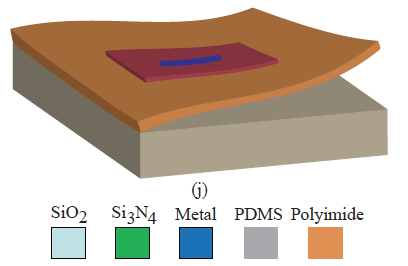
\includegraphics[width=\linewidth]{images/Traditional}
  \caption{A traditional arrangement and material breakdown of a durable tactile}
  \label{fig:Traditional}
\end{figure}

The current materials being implemented are P(VDF-TrFE) soft piezoelectric polymer films \cite{billard2013roboskin} \cite{dahiya2010tactile} These polymers demonstrate viscoelastic, and dielectric losses, which are used as an advantage to the substrate \cite{tinku2016micro} 

Stretchable polymers are a great means for rigidity and deformation, however its materials lack in the ability to conduct electrical signals efficiently \cite{yogeswaran2015new} \cite{rogers2010materials} Therefore conductive fillers were introduced to aid the conductivity of layers. 

This is a trade-off of course as the higher ratio of filler added, the less ductile the material, the more brittle the nano-wires \cite{billard2013roboskin} which of course is reliant for the system.


%Technological, social, economical and environmental impacts
\subsection{Social, Economical and Environmental impact}

The way in which fundamental interactions with the environment can be defined is limited. This interaction can be assessed in any necessary way in respect to a touch sense but without scientific method remains critique. 

The definitive method is the effects with peoples social interaction and ethics which is something to be further developed however is been found accepted in a general sense \cite{yogeswaran2015new}

The manufacturing process of the lamination is low cost which leads higher margins for profit gain and potentially affordable for a largely accepted market. 

As the research is applicable in more then several key developing areas the investment strategy and target market is fairly open for the picking, which gives much room for investor opportunity.

\clearpage
\subsection{Printable Materials}

The process of which a printable tactile can be established involves first moulding a cast with lithography, then inking by spin coating a wafer with composite ink and transferring that via the mould to another substrate, passing that substrate to polydimethylsiloxane (PDMS) cast and cure, and finally resulting with a patterned composite PDMS block. \cite{yogeswaran2015new} \cite{khan2015technologies}

\begin{figure}[h!]
  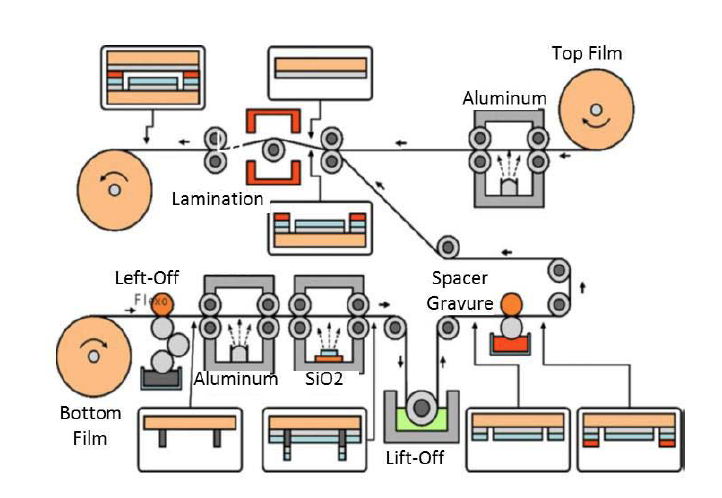
\includegraphics[width=\linewidth]{images/Process1}
  \caption{A general process of manufacturing diagram showing the stages a lamination is processed}
  \label{fig:Process1}
\end{figure}

\begin{figure}[h!]
  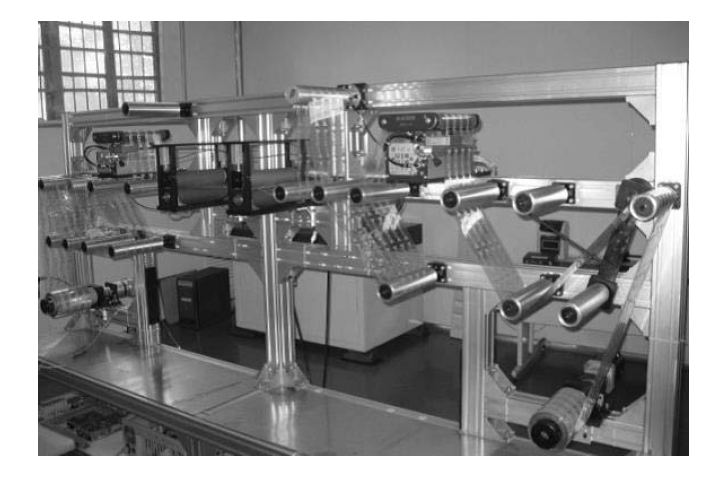
\includegraphics[width=\linewidth]{images/Process2}
  \caption{A processing equipment for a MOSFET tactile based on the previous diagram}
  \label{fig:Process2}
\end{figure}

Organic semiconductors are capable of meeting high-performance standards, however are such unstable \cite{dahiya2013bendable} As a result they can often be slower then an inorganic components. Further investigation for single crystal Si ultra graphene chips are in the early stages but hold promise \cite{yogeswaran2015new} 

\begin{figure}[h!]
  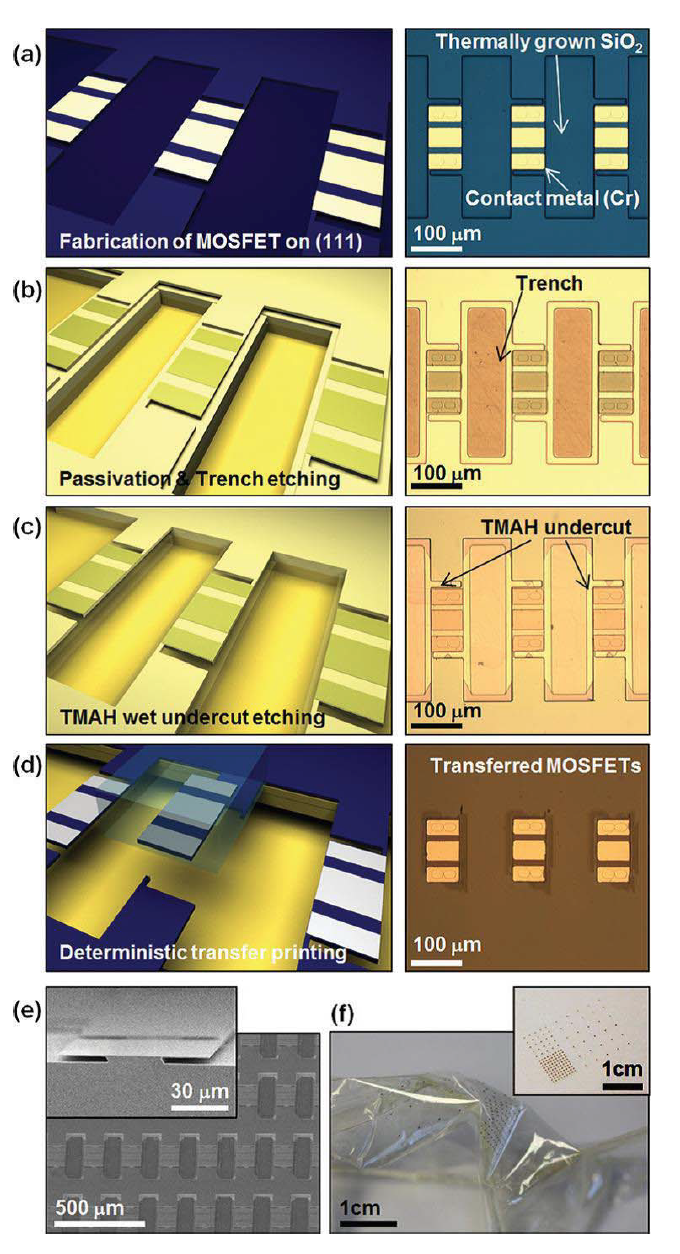
\includegraphics[width=\linewidth]{images/Durable}
  \caption{Composite PDMS block's (ink mould printed on to the film) in an array of elements and the final lamination}
  \label{fig:Durable}
\end{figure}

\subsection{Sensor Arrays}
In a standard manufacturing process, arrays of tactile's are printed in layers. These wafer thin layers (700 �m - 50 �m) form together in a combination of patterns of which a lining process envelopes a lamination \cite{yogeswaran2015new} that similar to skin but rather comprised of several parts silicon. Although silicon has become a popular and widely used material for tactile's in many research development centres around the world \cite{dahiya2013bendable}; Dr. Ravinder S. Dahiya has applied graphene in substitute as a filler for several prototypes in 2104.

While this method is not relatively new, it has been avoided in more of the films designs from methods produced by Rodolfo Zunino, and Maurizio Valle. The argument is that introducing graphene in the substrate is adding limitations on future development, but its important to note that the Si compounds widely used are mostly artificial, and therefore cost effective \cite{dahiya2007posfet} 

In order to produce a feasible method without the graphene, organic materials must first be further explored, to provide a more stable and cost effective approach \cite{dahiya2013posfet} Currently the organic materials although highly accurate, are highly unstable.

\begin{figure}[h!]
  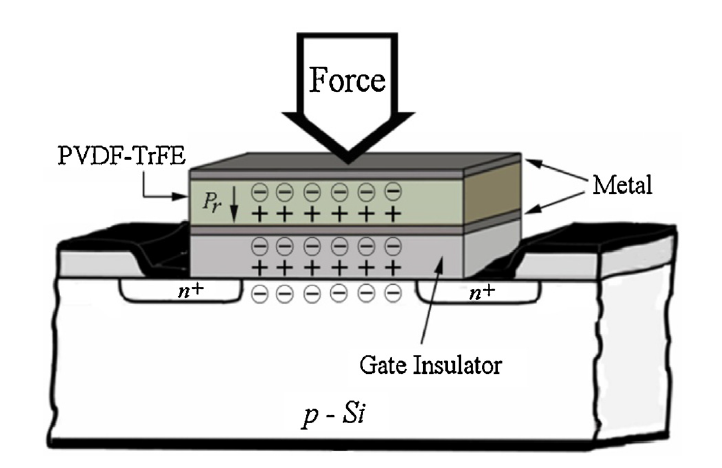
\includegraphics[width=\linewidth]{images/SingleElement}
  \caption{Single element diagram of a POSFET tactile}
  \label{fig:SingleElement}
\end{figure}

The ultra thin layers of each transistor are grown even smaller then other silicone-based types, Down to the micro scale for each piezoelectric oxide semiconductor field effect transistor (POSFET) \cite{yogeswaran2015new} 

Each element in the array generates a charge voltage, as per design of the MOSFET the signal is then amplified to be analysed by computational intelligence.

\begin{figure}[h!]
  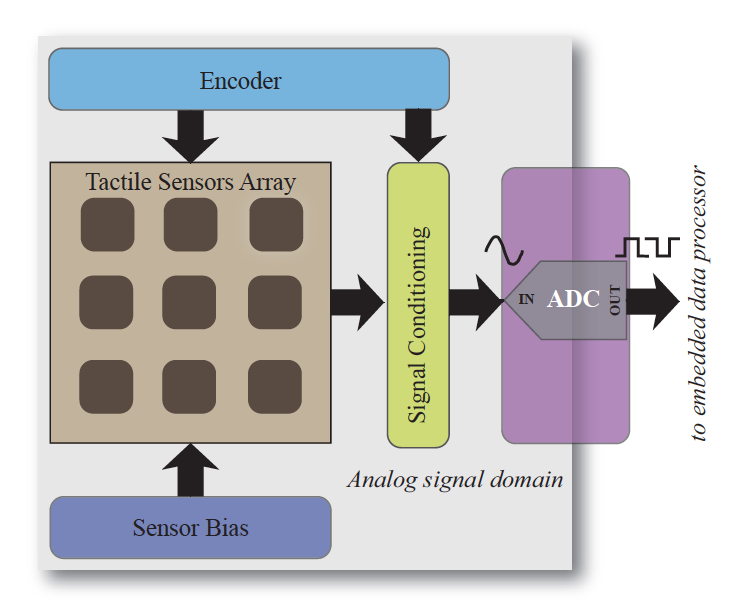
\includegraphics[width=\linewidth]{images/Array1}
  \caption{Sensor process diagram, how the signal is processed from each element in the array, then encoded and conditioned and passed to an ADC output}
  \label{fig:Array1}
\end{figure}

The CMOS Sensor Array consists of elements in the 32 micro electrode gates and are layered between 15 �m and 100 �m piezoelectric films \cite{khan2015technologies} \cite{dahiya2010tactile} \cite{dahiya2008tactile}

These films use an epoxy where higher filler of graphene is found \cite{dahiya2013posfet} The advantage is that each piezoelectric block has a higher control gain over the individual sensors and therefore simulated response when passed through as RAW data to the computational intelligence it's far more accurate \cite{dahiya2007posfet}

\begin{figure}[h!]
  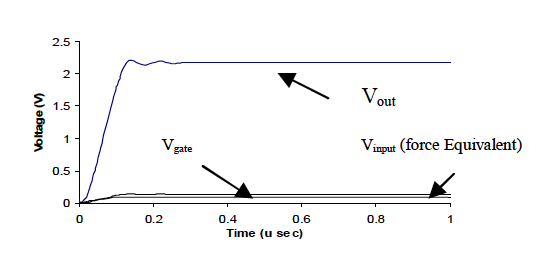
\includegraphics[width=\linewidth]{images/Sim}
  \caption{Simulated response comparison in CMOS 32 array of the applied force load and the voltage with respect to time, notice the low end interference and how this is negligible due to the classification type}
  \label{fig:Sim}
\end{figure}

\begin{figure}[h!]
  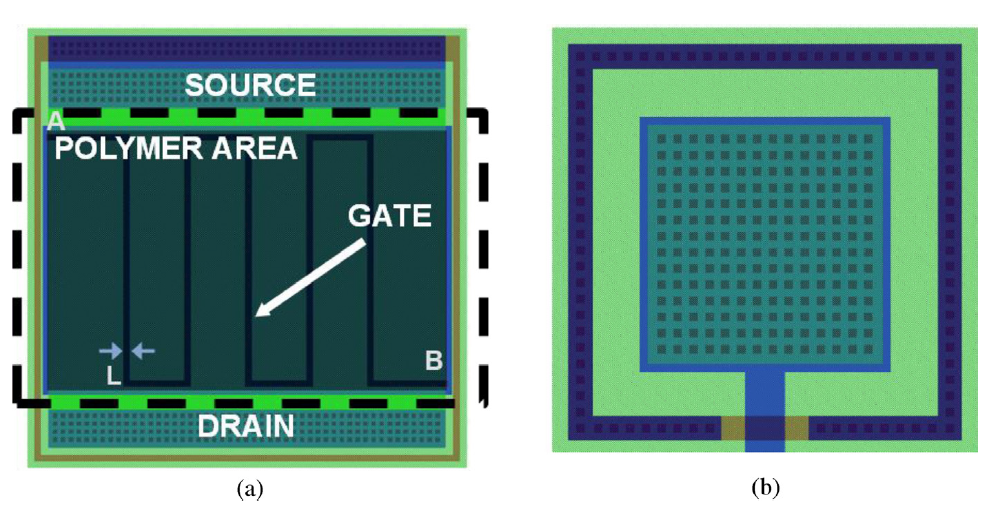
\includegraphics[width=\linewidth]{images/POSFET}
  \caption{POSFET Touch Sensor diagram a) Transistor Element b) 32 bit Array Formation}
  \label{fig:POSFET}
\end{figure}

Articles of Dr. Dahiya's more recent work discuss how the nano fabricated arrays are now using some of the graphene layers as conductive solar cells which are sufficient in self powering, they are also surprisingly \clearpage stable even in low light conditions (greater then 30\%). However the power is not enough for any computational processing.

While the arrays are fundamentally sound and produce a good response, they are not great and there is a long way to go as far as high definition in the resolution for the sense.

%\clearpage
\subsection{Computational Intelligence}

As a general rule the piezoelectric polymer transducer is influenced by types of materials on all sides. This is important to note when handling the RAW data. 

Computational intelligence introduces different approaches on how to deal with such information as well as how to deal with roughness, angled contact, also texture pattern recognition, and other object detection \cite{decherchi2011tactile} 	

Classifiers are used for the platform to address the dynamic range of forces \cite{cannata2010tactile} To calibrate this range, an instance of neural networks are stabilised using a learning machine; this uses probes of different materials and forces to generate a dynamic force range. 

The RAW data is passed to check the phase difference between each sensor on a difference deformation level, which is then used to average the force on the entire measurable area (like mapping how skin ranges from tight and stretchy, to hard and wrinkly) \cite{dahiya2010tactile}

Piezoelectric polymer properties offer a great range of positive aspects; however there are some drawbacks with factors to take account for, such as viscoelastic, dielectric losses. To compensate for these losses complex constants are in place for the elastic region, and often the phase of the signal must be classified with the dynamic forces \cite{kaboli2016novel}

\begin{figure}[h!]
  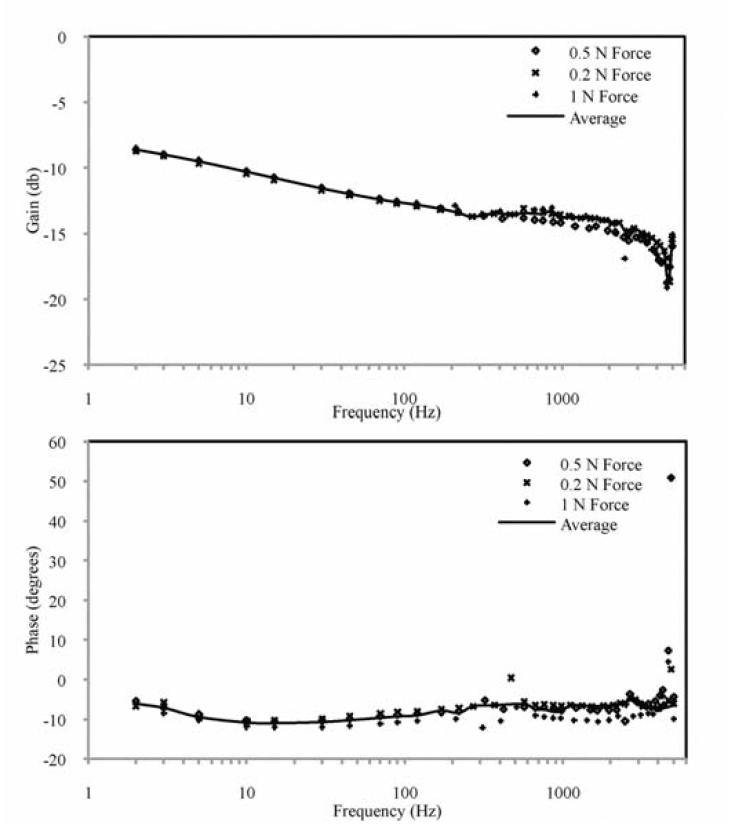
\includegraphics[width=\linewidth]{images/Posstruct}
  \caption{Phase and Gain plots at 3 different applied forces for MEA film}
  \label{fig:Posstruct}
\end{figure}

\subsection{Objects Orientation and Deformation}

Simultaneous localisation and mapping (SLAM) provides tactile arrays to demonstrate how the sensors can work in neural networks in order to use combine and predict algorithms, such that a 3D map of force over an object can be achieved \cite{dahiya2013directions} 

This technique relies on the stretchable surfaces and the inductance of the transducers being constant over a dynamic scale, and is therefore calculated using three formulas relating to the force over the array in simultaneous directions at any given time \cite{kaboli2016tactile} 	

\begin{figure}[h!]
  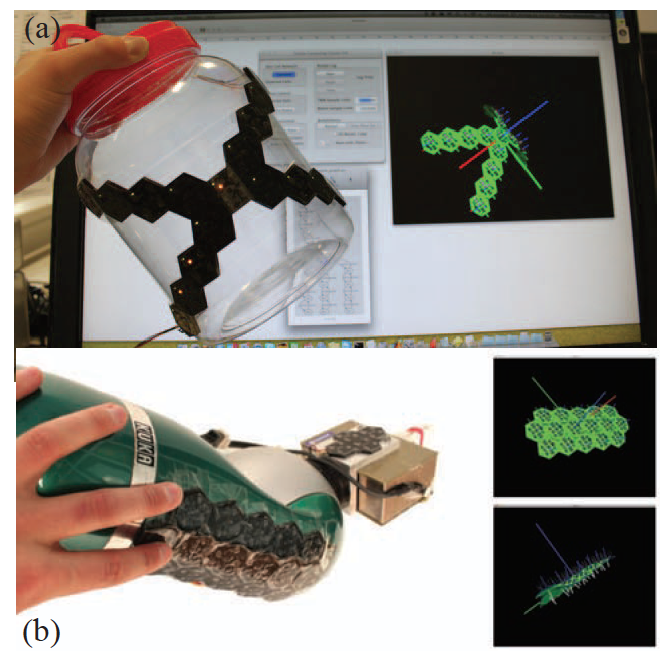
\includegraphics[width=\linewidth]{images/Demo}
  \caption{Simulation of POSFET type sensors over objects to produce a digital 3d map render of where the tactile's are positioned relative to one another}
  \label{fig:Demo}
\end{figure}

\clearpage
This technology is in its infancy stage and will be a few more years before implemented in the POSFET tactile system. The advantage of this is that with integration the signal elements can process sensing in live time, with predictions as to where applied forces will occur in advanced when clasping different objects. 

When a bottle or cup is picked up, majority of forces occur in four places; the bottom of the hand, the thumb, the fore-thumb and along the finger tips \cite{dahiya2013bendable} By using SLAM with the tactile's, predictions can be made as to what object is about to be obtained and what forces to expect. 

Further advantage of using this process is that while a large dynamic range may not be available in one calibrated setting; the array gives opportunity to adjust the calibration dependent on the predicted forces expected. \cite{kaboli2015hand} 


\begin{comment}
This part here does this and this and this, this other part does this and this but we want to achieve this and this so we have chosen this sensor.

These sensors won't work because of this and these sensors are ok for this but here are the faults

Find where the research leads to and present it in that way for the end product and explaining things.

This is what the guy was explaining and not pulling things out of the sky.

Critical analysis
- Evaluate relevant research done by other researchers by ? Determining strengths and weaknesses of methods,
results, conclusions and recommendations ? Expressing and justifying agreement and disagreement
\end{comment}

%\clearpage
\section{CONCLUSIONS}

The results are highly influenced by real-world factors. How it feels when touched to a surface can be dependent on a number of considered reasons; these include interaction behaviours when the tactile's are deformed \cite{cannata2010modular} 

Contact to objects and other external forces are not exempt to the noise of motion; meaning that not only the weight of an object and its deformation to the sensors must be compensated, but also how the motion and movements change this dynamic measurement. 

If the array were to sense a spiky ball being held in place, then squeezed the ball, and lastly push and roll the ball on a 3rd surface; the sensitivity of forces are calibrated such that an array can concise of 25 to 256 elements, thus providing a comparable use of range \cite{dahiya2013posfet}

It is found that with the current range of research POSFET element, CMOS arrays are at a strong point and have future development underway with 3D mapping and force prediction \cite{cannata2010tactile} The POSFET tactile's are to a high enough resolution, and the durable, ductile material allows to be fitted to a specific or wide range of applications.

The properties of the piezoelectric blocks are stable enough and provide an accurate dynamic range of feedback, which when using correct classification and accounting for the phase and gain with deformation, will provide a close to life like sense similar to that of a human hand \cite{dahiya2009development}

The material is also 98.78\% translucent, and remarkably thin, allowing the application to be used as a medicine glove, or other low profile device for a wide range of applications \cite {yogeswaran2015new} The limitations at this stage are that it is not yet an everyday usable device, and may not be available for commercial application for some time. 

The major setback is if a single element becomes offline the series will fail, and due to the inability to change individual components the entire unit would need to be replaced; however with respect to the cost per unit, this is considerably cheap to manufacture \cite{billard2013roboskin}

For the purpose of this task, the piezoelectric array tactile's, PRINTSKIN (Dr. Ravinder S. Dahiya, University of Glasgow Scotland) or E-Skin (Tokyo University Professor Takao Someya) is optimal for measuring the variety of difference between a sea egg or chicken egg. 


\begin{comment}
?	The conclusion summarises the key findings of the review in general terms. Notable similarities between works, whether favourable or not, may be included here.
?	This section is the reviewer's opportunity to justify a research proposal. Therefore, the idea should be clearly re-stated and supported according to the findings of the review.
\end{comment}


%\addtolength{\textheight}{-12cm}   % This command serves to balance the column lengths


%\section*{APPENDIX}

\begin{comment}
?	As well as accurate in-text citations, a literature review must contain complete and correct citations for every source.

Referencing
o No plagiarism (all borrowed material must be adequately referenced).
o Consistent use of citation style throughout the chapter o Complete reference list

\begin{itemize}
	\item Be thorough and inclusive of all details concerning the decision 
	\item Be objective and not subjective to details central to the project
	\item Be aware of what the decision means or the outcome of the project
\end{itemize}	

\end{comment}

\clearpage
\section*{ACKNOWLEDGMENT}

\nocite{*}
\bibliographystyle{ieeetr}
\bibliography{references}

\end{document}
